% file: modeledsystems.tex

\chapter{Modeled systems}
This chapter contains descriptions of the systems that I have modeled durung my Master project. 
\section{Bulk S1 hydrate}
\subsection{Elastic properties}
To my knowledge, there are no published estimates of Youngs modulus and the Poisson ratio for the TIP4P/ICE+UAM model of methane hydrates. Therefore, I seek to make crude estimates of these quantities in dynamic simulations. I apply a constant strain rate by continously rescaling particle positions in one direction during MD-simulations. The other directions are kept under a constant pressure with anisotropic barostatting. Figure \ref{fig:stress_strain_11_11_11_tip4p_ice_uam} shows the stress strain relationships and corresponding estimates of Youngs modulus for a system of 11x11x11 S1 unit cells subjected to strain rates of \SI{5d-7}{\per\femto\second} and \SI{2d-7}{\per\femto\second}. By extrapolating the results to quasistatic strain, Youngs modulus is estimated to \SI{7.1}{\giga\pascal}.

\begin{figure}
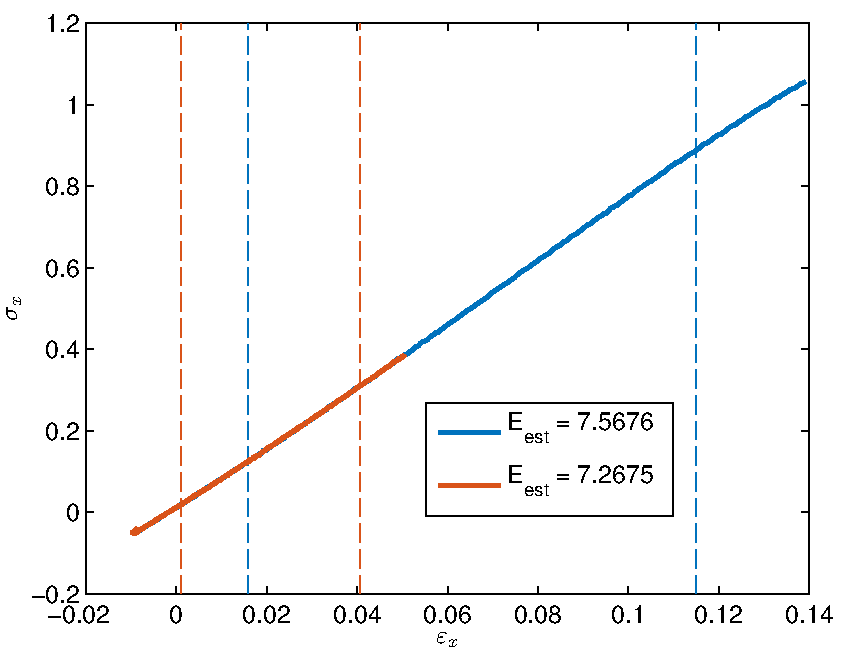
\includegraphics[width=12cm]{../figures/thesis/stress_strain_11_11_11_tip4p_ice_uam.pdf}
\caption{Stess-strain relations for a system of 11x11x11 S1 unit cells. Dashed lines indicate the region that was used to estimate Youngs modulus. Strain rates of \SI{5d-7}{\per\femto\second} (blue) and \SI{2d-7}{\per\femto\second} (red) along the x-axis.}
\label{fig:stress_strain_11_11_11_tip4p_ice_uam}
\end{figure}

\section{Vega 2010}
\section{Determining the critical stress intensity factor}
As described in the section about fracture mechanics, the stress intensity factor is commonly used to calculate the fracture toughness of a material. Assuming methane hydrates to be brittle (which jush might be a good assumption), I use fracture theories developed by Griffiths to estimate the stress intensity factor for S1 methane hydrate. I cut a 

